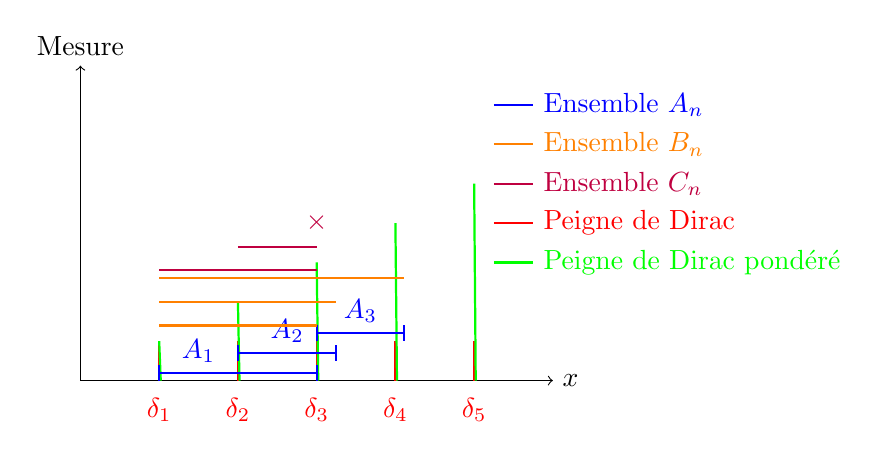
\begin{tikzpicture}
    % Axes
    \draw[->] (0,0) -- (6,0) node[right] {$x$};
    \draw[->] (0,0) -- (0,4) node[above] {Mesure};

    % Peigne de Dirac
    \foreach \x in {1,2,3,4,5} {
        \draw[red, thick] (\x,0) -- (\x,0.5);
        \draw[red] (\x,-0.1) node[below] {$\delta_{\x}$};
    }

    % Peigne de Dirac pondéré
    \foreach \x in {1,2,3,4,5} {
        \draw[green, thick] (\x+0.02,0) -- (\x,\x*0.5);
    }

    % Intervalles A_n
    \draw[blue, thick] (1.5,0.1) node[above] {$A_1$};
    % base line
    \draw[blue, thick] (1,0.1) -- (3,0.1);
    % edges
    \draw[blue, thick] (1,0.2) -- (1,0);
    \draw[blue, thick] (3,0.2) -- (3,0);


    \draw[blue, thick] (2,0.35) -- (3.25,0.35) node[midway, above] {$A_2$};
    % edges
    \draw[blue, thick] (2,0.45) -- (2,0.25);
    \draw[blue, thick] (3.25,0.45) -- (3.25,0.25);


    \draw[blue, thick] (3,0.6) -- (4.11,0.6) node[midway, above] {$A_3$};
    % edges
    \draw[blue, thick] (3,0.7) -- (3,0.5);
    \draw[blue, thick] (4.11,0.7) -- (4.11,0.5);

    % Intervalles B_n
    \draw[orange, thick] (1,0.7) -- (3,0.7);
    \draw[orange, thick] (1,1) -- (3.25,1);
    \draw[orange, thick] (1,1.3) -- (4.11,1.3);

    % Intervalles C_n
    \draw[purple, thick] (1,1.4) -- (3,1.4);
    \draw[purple, thick] (2,1.7) -- (3,1.7);
    \draw[purple] (3,2) node[circle] {$\times$};

    % Légende
    \draw[blue, thick] (5.25,3.5) -- (5.75,3.5) node[right] {Ensemble $A_n$};
    \draw[orange, thick] (5.25,3) -- (5.75,3) node[right] {Ensemble $B_n$};
    \draw[purple, thick] (5.25,2.5) -- (5.75,2.5) node[right] {Ensemble $C_n$};
    \draw[red, thick] (5.25,2) -- (5.75,2) node[right] {Peigne de Dirac};
    \draw[green, thick] (5.25,1.5) -- (5.75,1.5) node[right] {Peigne de Dirac pondéré};
\end{tikzpicture}